\documentclass[12pt]{article}
%% arXiv paper template by Flip Tanedo
%% last updated: Dec 2016



%%%%%%%%%%%%%%%%%%%%%%%%%%%%%
%%%  THE USUAL PACKAGES  %%%%
%%%%%%%%%%%%%%%%%%%%%%%%%%%%%

\usepackage{amsmath}
\usepackage{amssymb}
\usepackage{amsfonts}
\usepackage{graphicx}
\usepackage{xcolor}
\usepackage{nopageno}
\usepackage{enumerate}
\usepackage{parskip}

%%%%%%%%%%%%%%%%%%%%%%%%%%%%%%%%%
%%%  UNUSUAL PACKAGES        %%%%
%%%  Uncomment as necessary. %%%%
%%%%%%%%%%%%%%%%%%%%%%%%%%%%%%%%%

\usepackage{tikzfeynman}

\usepackage{titlesec}
\titleformat*{\section}{\large\bfseries}

%% MATH AND PHYSICS SYMBOLS
%% ------------------------
%\usepackage{slashed}       % \slashed{k}
%\usepackage{mathrsfs}      % Weinberg-esque letters
%\usepackage{youngtab}	    % Young Tableaux
%\usepackage{pifont}        % check marks
\usepackage{bbm}           % \mathbbm{1} incomp. w/ XeLaTeX 
%\usepackage[normalem]{ulem} % for \sout


%% CONTENT FORMAT AND DESIGN (below for general formatting)
%% --------------------------------------------------------
\usepackage{lipsum}        % block of text (formatting test)
%\usepackage{color}         % \color{...}, colored text
%\usepackage{framed}        % boxed remarks
%\usepackage{subcaption}    % subfigures; subfig depreciated
%\usepackage{paralist}      % compactitem
%\usepackage{appendix}      % subappendices
%\usepackage{cite}          % group cites (conflict: collref)
%\usepackage{tocloft}       % Table of Contents	

%% TABLES IN LaTeX
%% ---------------
%\usepackage{booktabs}      % professional tables
%\usepackage{nicefrac}      % fractions in tables,
%\usepackage{multirow}      % multirow elements in a table
%\usepackage{arydshln} 	    % dashed lines in arrays

%% Other Packages and Notes
%% ------------------------
%\usepackage[font=small]{caption} % caption font is small



%\renewcommand{\thesection}{}
%\renewcommand{\thesubsection}{\arabic{subsection}}

%%%%%%%%%%%%%%%%%%%%%%%%%%%%%%%%%%%%%%%%%%%%%%%
%%%  PAGE FORMATTING and (RE)NEW COMMANDS  %%%%
%%%%%%%%%%%%%%%%%%%%%%%%%%%%%%%%%%%%%%%%%%%%%%%

\usepackage[margin=2cm]{geometry}   % reasonable margins

\graphicspath{{figures/}}	        % set directory for figures

% for capitalized things
\newcommand{\acro}[1]{\textsc{\MakeLowercase{#1}}}    

\numberwithin{equation}{section}    % set equation numbering
\renewcommand{\tilde}{\widetilde}   % tilde over characters
\renewcommand{\vec}[1]{\mathbf{#1}} % vectors are boldface

\newcommand{\dbar}{d\mkern-6mu\mathchar'26}    % for d/2pi
\newcommand{\ket}[1]{\left|#1\right\rangle}    % <#1|
\newcommand{\bra}[1]{\left\langle#1\right|}    % |#1>
\newcommand{\Xmark}{\text{\sffamily X}}        % cross out

% Change list spacing (instead of package paralist)
% from: http://en.wikibooks.org/wiki/LaTeX/List_Structures#Line_spacing
%\let\oldenumerate\enumerate
%\renewcommand{\enumerate}{
%  \oldenumerate
%  \setlength{\itemsep}{1pt}
%  \setlength{\parskip}{0pt}
%  \setlength{\parsep}{0pt}
%}

\let\olditemize\itemize
\renewcommand{\itemize}{
  \olditemize
  \setlength{\itemsep}{1pt}
  \setlength{\parskip}{0pt}
  \setlength{\parsep}{0pt}
}


% Commands for temporary comments
\newcommand{\comment}[2]{\textcolor{red}{[\textbf{#1} #2]}}
\newcommand{\flip}[1]{{\color{red} [\textbf{Flip}: {#1}]}}
\newcommand{\email}[1]{\texttt{\href{mailto:#1}{#1}}}

\newenvironment{institutions}[1][2em]{\begin{list}{}{\setlength\leftmargin{#1}\setlength\rightmargin{#1}}\item[]}{\end{list}}


\usepackage{fancyhdr}		% to put preprint number



% Commands for listings package
\usepackage{listings}      % \begin{lstlisting}, for code
%
 \lstset{basicstyle=\ttfamily\footnotesize,breaklines=true}
%    sets style to small true-type


%%%%%%%%%%%%%%%%%%%%%%%%%%%%%%%%%%%%%%%%%%%%%%
%%%  TIKZ COMMANDS FOR EXTERNAL DIAGRAMS  %%%%
%%%  requires -shell-escape               %%%%
%%%  in texpad 1.7: prefs > shell esc sec %%%%
%%%%%%%%%%%%%%%%%%%%%%%%%%%%%%%%%%%%%%%%%%%%%%

%% This is for exporting tikz figures as into a ./tikz/ subfolder.
%% It is useful if you want pdf versions of the tikz diagrams or
%% if you need to speed up compilation of a large document with
%% many tikz diagrams.

%\write18{} % Careful with this!
%\usetikzlibrary{external}
%\tikzexternalize[prefix=tikz/] % folder for external pdfs


%%%%%%%%%%%%%%%%%%%
%%%  HYPERREF  %%%%
%%%%%%%%%%%%%%%%%%%

%% This package has to be at the end; can lead to conflicts
\usepackage{microtype}
\usepackage[
	colorlinks=true,
	citecolor=black,
	linkcolor=black,
	urlcolor=green!50!black,
	hypertexnames=false]{hyperref}



%%%%%%%%%%%%%%%%%%%%%
%%%  TITLE DATA  %%%%
%%%%%%%%%%%%%%%%%%%%%

%%% PREPRINT NUMBER USING fancyhdr
%%% Don't forget to set \thispagestyle{firststyle}
%%% ----------------------------------------------
%\renewcommand{\headrulewidth}{0pt} % no separator
%\fancypagestyle{firststyle}{
%\rhead{\footnotesize \texttt{UCI-TR-2016-XX}}}



\begin{document}

%\thispagestyle{empty}
%\thispagestyle{firststyle} %% to include preprint

\begin{center}

    {\Large \textsc{Homework 6:} 
    \textbf{Fourier Review}}


    
\end{center}

\vskip .4cm

\noindent
\begin{tabular*}{\textwidth}{rlcrll}
	\textsc{Course:}& Physics 231, \emph{Methods of Theoretical Physics} (2017)
	&
%	\hspace{1.2cm}
	&
	\\
	\textsc{Instructor:}& Flip Tanedo (\email{flip.tanedo@ucr.edu})
	&
	%\hfill
	&
	& 
	\\
	\textsc{Due by:}& Friday, November 10
	&
	%\hfill
	&
	%	
\end{tabular*}



\textbf{Reading}: For this week, make sure you understand the example we did in Lecture 15:
\begin{align*}
	\int_{-\infty}^\infty dx \; \frac{2\cos x}{x^2+1} \ .
\end{align*}
This week we're pivoting back towards Green's functions now that we are armed with the power of the residue theorem. I will be assuming that you are familiar with \textbf{Fourier transforms}, if Problem 1 of this homework is not straightforward, please review them. Here are some references you may consider following:
\begin{itemize}
	\item \textsc{Boas} (3rd ed): Chapters 7.7 (complex form of Fourier series), 7.12 (Fourier transforms), 8.12 (Green's functions)
	\item \textsc{Appel}: Chapters 4.6.c (Fourier integrals), 10 (Fourier transforms), 13 (Physical applications of the Fourier transform), 15 (Green's functions, especially 15.2.b)
	\item \textsc{Matthews \& Walker} (2nd ed): Chapters 4.2 (Fourier transforms), 5.2 (Dispersion relations), 9 (Green's functions)
	\item \textsc{Byron \& Fuller}:  Chapters 5.7 (Fourier integrals; note that they use different conventions than we do---this is why Problem 1 is important for us), 6.6 (Dispersion relations), 7 (Green's functions)
\end{itemize}

We will have discussion section on Monday at 3:10pm in Chung 142. This is completely optional\footnote{For the record, lectures are also optional.}, but I welcome you to come to ask questions about the homework or the course at large. 




\section{A Fourier transform refresher}
%https://physics.stackexchange.com/questions/308234/fourier-transform-standard-practice-for-physics/308252

Fourier transforms are annoying because there are a few choices that one has to make to establish conventions. The convention that we will use is: % consistent with Peskin
\begin{align}
	f(x) &= \int \frac{dk}{2\pi} e^{-ikx}\, \tilde f(k)
	&
	\tilde f(k) &= \int dx \, e^{ikx}\, f(x) \ .
\end{align}
In this convention, the $(2\pi)$ comes with the $dk$, so I will often write $\dbar k = dk/(2\pi)$.

\subsection{Fourier decomposition of $\delta(x)$}

What is the Fourier transform of $\delta(x)$? In other words, find $\tilde \delta(k)$ in
\begin{align}
	\delta(x) = \int \dbar k \, e^{ikx}\, \tilde\delta(k) \ .
\end{align}
What about $\delta(x-x_0)$?

\subsection{Other conventions}
%https://physics.stackexchange.com/questions/308234/fourier-transform-standard-practice-for-physics

A general convention for the Fourier transform is:
\begin{align}
	f(x) &= |B|^{1/2}
	\int \frac{dk}{\sqrt{(2\pi)^{1+A}}} \, e^{-iBkx} \tilde f(k)
	&
	\tilde f(k) &= |B|^{1/2}
	\int \frac{dx}{\sqrt{(2\pi)^{1-A}}} \, e^{iBkx} f(x) \ .
\end{align}
Our conventions correspond to $B=1$ and $A=1$. Show that in this general form, the inverse Fourier transform of a Fourier transform is simply the original function. 

\subsection{Higher dimensions}

In two Euclidean dimensions, the Fourier transform is
\begin{align}
	f(x, y) = \int\frac{dx}{2\pi} \int\frac{dy}{2\pi} \, e^{-ik_xx} e^{-ik_yy} \tilde f(k_x, k_y) \ .
\end{align}
This can be rewritten in terms of a position 2-vector\footnote{Mathematicians laugh at us when we say `position vector.'} $\vec{x}$ and corresponding momentum 2-vector $\vec{k}$ \ , 
\begin{align}
	f(\vec x) = \int\frac{d^2\vec x}{(2\pi)^2}  \, e^{-i\vec k\cdot \vec y} \tilde f(\vec k) \ .
\end{align}
Observe that the exponential is built out of the rotationally-invariant scalar quantity, $\vec k\cdot \vec y$. 
%
When we deal with \emph{partial} differential equations, we'll need to Fourier transform in multiple dimensions. Sometimes we'll have to Fourier transform in both time and space. It is conventional to choose signs so that we may write this as 
\begin{align}
	f(x, t) = \int\frac{dx}{2\pi} \int\frac{dt}{2\pi} \, e^{+ikx} e^{-i\omega t} \tilde f(k, \omega) \ .
\end{align}
Briefly comment why this is a good idea from two points of view:
\begin{enumerate}
	\item The idea that we are expanding about a basis of traveling plane waves. 
	\item Lorentz invariance, in case we want our expressions to respect special relativity.
\end{enumerate}

\section{Integral representation of the step function}
% Cahill Problem 5.32

[\textsc{Cahill}, Problem 5.32] 
The step function is defined by $\Theta(x) = 0$ for $x<0$ and $\Theta(x) = 1$ for $x>0$. Show that this is equivalent to
\begin{align}
	\Theta(x) = \frac{1}{2\pi i}\int_{-\infty}^\infty \frac{e^{ixz}}{z-i\varepsilon} dz \ .
\end{align}

\textsc{Hint}: What does the $-i\epsilon$ mean? Compare this to the advanced and retarded Green's functions that we explored in Lecture 15. 



\appendix
\section*{\Large Extra Credit}


These problems are not graded and are for your edification. You are strongly encouraged to explore and discuss these topics, especially if they are in a field of interest to you.

\section{The Riemann Sphere}

% explain why you don't worry about edge effects, but you should worry about a pole at infinity

[\textsc{Appel} Section 5.4]
%
In class we introduced the idea of the \textbf{Riemann sphere} in the context of whether there could be `edge effects' when converting an integral along $\mathbb{R}$ to a closed contour in the complex plane.
The Riemann sphere is a completion of the complex plane that include the point at infinity. That is to say, $\infty = R e^{i\theta}$ as $R\to$ `very big' and for any $\theta$. Note that this means $i\infty \equiv \infty$. 

The mapping is demonstrated below (image from Boas, \emph{Mathematical Methods in the Physical Sciences}):

\begin{center}
% Image from Boas
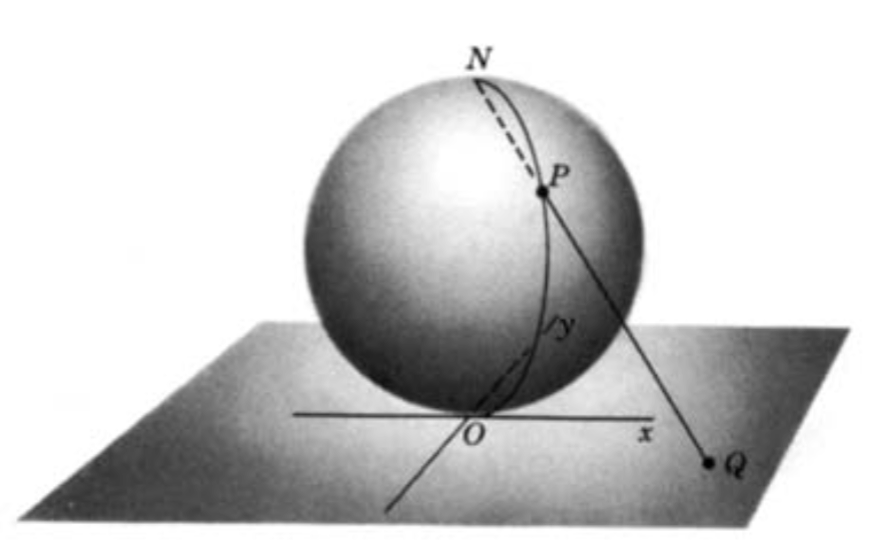
\includegraphics[width=.5\textwidth]{Boas_RiemannSphere}	
\end{center}

Imagine a sphere situated at the origin, $O$ of the complex plane. The north pole of the sphere, $N$, is our reference point. Any point on the complex plane $Q$ is mapped to a point $P$ on the Riemann sphere given by the intersection of the line $NQ$ with the sphere. Infinity is identified with $N$. Observe that an integral along the real line has an integral around the Riemann sphere. Also note that the notion of ``inside'' versus ``outside'' becomes somewhat slippery\footnote{A physicist and a mathematician are asked to optimize the amount of land inside a fence of fixed length, $L$. The physicist deduces that enclosing a circular region with radius $R = L/2\pi$ optimizes the area enclosed. The mathematician sees a flaw in this logic and subsequently throws away most of the fence and encloses a circle of size $r \ll R$. The mathematician steps inside tiny region and says, ``I declare myself to be on the outside.'' }. A useful convention is that `inside' is to the left of the direction of the contour\footnote{Note how \emph{orientation} avoids the issue raised in the above footnote.}. 

\begin{enumerate}[(a)]
\item Show that the residue of a function $f$ at $\infty$ is 
\begin{align}
\text{Res}(f,\infty) = \text{Res}\left(-\frac{f(1/z)}{z^2},0\right),
\end{align}
\textsc{Hint}: we don't understand how to deal with a pole at $\infty$, so map that pole to a pole that's somewhere on the complex plane. Be sure to explain the sign.
\item Imagine a small curve $C$ that loops once around a point $P$ somewhere `in the middle' in the Riemann sphere, as shown above. We know that $f(z)=1/z$ is analytic in this region, so $\oint_C f(z) dz = 0$. However, if we reverse the orientation of the curve $C$ and follow the `inside is to the left' rule, this curve now encloses the pole at $z=0$ which has $\text{Res}(f,0) = 1$. If we're just taking $C \to -C$, we expect the integral to flip signs. How does this result make sense?
\textsc{Hint}: What is the residue of $f(z) = 1/z$ at infinity?
\end{enumerate}
% From Appel, 5.4




\end{document}